\subsection{Referencias}

Se presenta un listado de los conectores y notación especial utilizada en los diagramas, a modo de referencia. Además se provee el zoom sobre algunos conectores especiales.

\begin{figure}[H]
   \centering
   \includegraphics[width=\textwidth]{reentrega/imagenes/referencias1.png}
   \caption{Referencias de diagramas (Parte 1).}
\end{figure}

\newpage

\begin{figure}[H]
   \centering
   \includegraphics[width=\textwidth]{reentrega/imagenes/referencias2.png}
   \caption{Referencias de diagramas (Parte 2).}
\end{figure}

\subsubsection{Client-Server Seguro (SSL)}

La comunicación segura via SSL funciona de la siguiente manera. Supongamos que un cliente desea comenzar una comunicación segura con un servidor.

En primer lugar, le solicita al servidor sus certificados SSL, para verificar la autoridad. Solicita tanto la clave pública como los certificados y los compara con los que tiene almacenados localmente.

En el siguiente paso, el servidor le solicita al cliente que genere un número random. El cliente genera el número, lo encripta utilizando la clave pública para que sea el servidor el único que pueda leerlo y se lo envía.

El servidor obtiene este número, lo desencripta utilizando su clave privada, y posteriormente utiliza el número aleatorio para generar una clave simétrica. La clave es encriptada mediante un algoritmo conocido por el cliente utilizando el número aleatorio, y luego utilizando la clave privada. El cliente utiliza la clave pública para resolver la primera enriptación, y luego el desencriptador con el mismo número aleatorio que le ha enviado al servidor. En este momento, ambas partes tienen la clave simétrica que utilizarán posteriormente para encriptar y desencriptar los pedidos y las respuestas.

Ambos almacenan la clave simétrica en repositorios para su posterior uso. La clave simétrico expira cada cierto tiempo, por lo que el protocolo debe volver a ejecutarse.


\newpage

\begin{figure}[H]
   \centering
   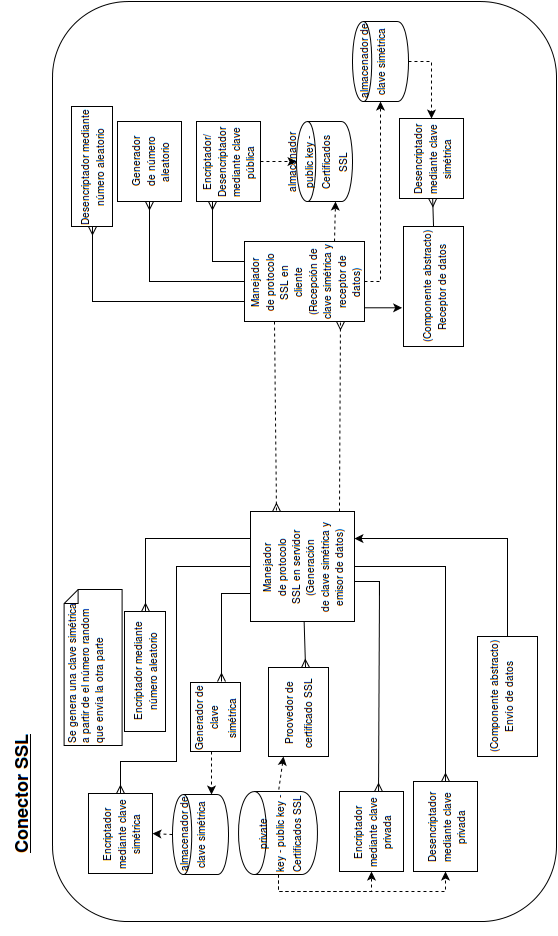
\includegraphics[height=0.95\textheight]{reentrega/imagenes/conector-ssl.png}
   \caption{Zoom de conector Client-Server Seguro (SSL).}
\end{figure}


\subsubsection{Client-Server Seguro con destinatario favorito}

\begin{figure}[H]
   \centering
   \includegraphics[width=\textwidth]{reentrega/imagenes/componente-cs-seguro-favorito.png}
   \caption{Zoom de conector Client-Server Seguro con destinatario favorito.}
\end{figure}

El componente Enviador/Receptor intenta enviar el mensaje
al destinatario favorito (Servidor) mediante SSL y setea un timer.
Si el timer avisa, es decir si se produce un timeout, el componente
cierra la sesión SSL creada previamente y busca al azar entre los
demás destinatarios posibles, y repite el proceso. El destinatario
favorito se marca como ``inaccesible'' y se setea un timer en 10
minutos que avisará al componente ``Habilitador de destinatario
favorito'' que vuelva a habilitar el destinario favorito para
futuro uso.

La idea es que si el destinatario favorito vuelve a ser accesible se
vuelva a utilizar, pero se le da un tiempo antes de reintentar para
no saturarlo y poder seguir operando sin que se produzca timeout
en todos los pedidos (a causa de que el favorito está caido).

\subsubsection{Client-Server Seguro con caché en el cliente}

\begin{figure}[H]
   \centering
   \includegraphics[width=\textwidth]{reentrega/imagenes/componente-cs-seguro-cache.png}
   \caption{Zoom de conector Client-Server Seguro con caché en el cliente.}
\end{figure}

El ``Resovedor de request HTTP'' primero busca el recurso en la caché:
\begin{itemize}
	\item Si no lo encuentra, busca el request entre los que fueron enviados pero aún no respondieron:
	\begin{itemize}
		\item Si no lo encuentra, de manera atómica escribe el request en ese repositorio para indicar a futuros
        pedidos que ese request será cacheado a la brevedad. Luego envía el request al ``Enviador/Receptor de
        request/response HTTP'', el cual lo envía al servidor. Cuando recibe la respuesta, la escribe en la caché
        y luego marca el request con el flag de ``Cacheado'' en el repositorio de requests HTTP enviados. Finalmente
        devuelve el response al ``Resolvedor de request HTTP'', que se lo retorna al cliente.
        
        \item Si lo encuentra, se suscribe al blackboard de Requests enviados que aún no respondieron.
        Cuando el flag de ese request pasa a estar en ``Cacheado'', se dispara el evento
        a todos los suscriptos para que sepan que ya está cacheado el pedido. Luego el ``Resolvedor de
        request HTTP'' busca el pedido en la caché.
	\end{itemize}
	
	\item  Si lo encuentra en la caché, simplemente lo retorna.
\end{itemize}

En paralelo, hay un proceso ``Purgador de caché'' que cada X tiempo configurable borra las entradas
de caché que en ese tiempo no hayan sido usadas o que tengan TTL=0.


\subsubsection{Client-Server Seguro con destinatario favorito y caché en el cliente}

\begin{figure}[H]
   \centering
   \includegraphics[width=\textwidth]{reentrega/imagenes/componente-cs-seguro-favorito-cache.png}
   \caption{Zoom de conector Client-Server Seguro con destinatario favorito y caché en el cliente.}
\end{figure}


El ``Resovedor de request HTTP'' primero busca el recurso en la caché:
\begin{itemize}
	\item Si no lo encuentra, busca el request entre los que fueron enviados pero aún no respondieron:
	\begin{itemize}
		\item Si no lo encuentra, de manera atómica escribe el request en ese repositorio para indicar a futuros
        pedidos que ese request será cacheado a la brevedad. Luego envía el request al ``Enviador/Receptor de
        request/response HTTP'', el cual lo envía al servidor. Cuando recibe la respuesta, la escribe en la caché
        y luego marca el request con el flag de ``Cacheado'' en el repositorio de requests HTTP enviados. Finalmente
        devuelve el response al ``Resolvedor de request HTTP'', que se lo retorna al cliente.
        
        \item Si lo encuentra, se suscribe al blackboard de Requests enviados que aún no respondieron.
        Cuando el flag de ese request pasa a estar en ``Cacheado'', se dispara el evento
        a todos los suscriptos para que sepan que ya está cacheado el pedido. Luego el ``Resolvedor de
        request HTTP'' busca el pedido en la caché.
	\end{itemize}
	
	\item  Si lo encuentra en la caché, simplemente lo retorna.
\end{itemize}

En paralelo, hay un proceso ``Purgador de caché'' que cada X tiempo configurable borra las entradas
de caché que en ese tiempo no hayan sido usadas o que tengan TTL=0.